\documentclass{beamer}

\usetheme{CambridgeUS}
\usecolortheme{orchid}

\usepackage{graphicx}
\usepackage{tikz}
\usepackage{listings}
\usepackage{colortbl}

\tikzstyle{block} = [rectangle, draw, text width=4.5em, text centered, minimum height=2em]
\lstset{basicstyle=\small\ttfamily}



\lstset{
  language=Java,
  basicstyle=\ttfamily\small,
  keywordstyle=\color{blue},
  commentstyle=\color{green!60!black},
  stringstyle=\color{red},
  showstringspaces=false,
  breaklines=true
}

\setbeamertemplate{navigation symbols}{} % Remove navigation symbols

\title{API Design and Management}
\author{Mohamed Sweelam}
\institute{Software Engineer}
\date{}

\begin{document}

\begin{frame}
  \titlepage
\end{frame}

\begin{frame}{Outline}
  \tableofcontents
\end{frame}

\section{Course Introduction}
\begin{frame}{Course Introduction}
  \begin{itemize}
    \item Overview of API Design and Management
    \item Role and Importance of APIs in Microservices and Distributed Systems
  \end{itemize}
\end{frame}

\section{Understanding APIs}
\begin{frame}{Understanding APIs}
  \begin{center}
    % 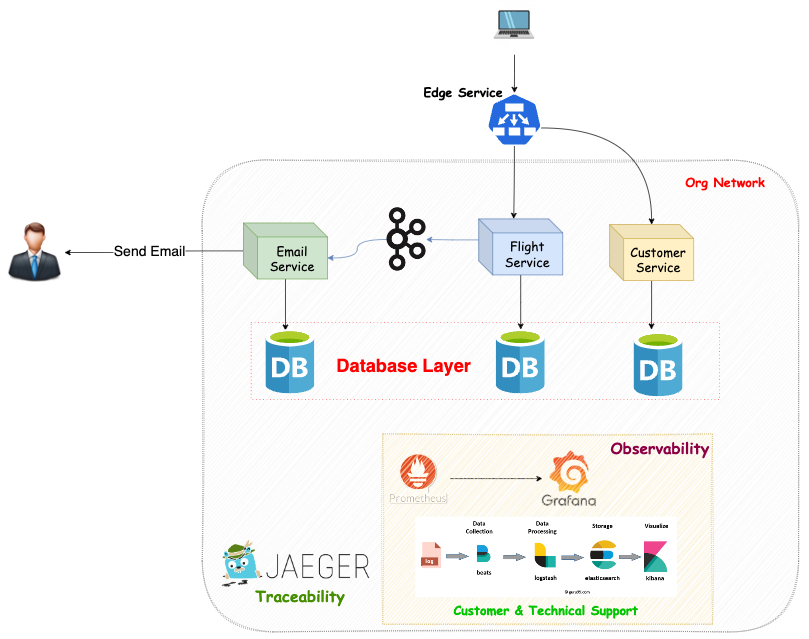
\includegraphics[width=0.7\textwidth]{img/system-HLD-1.png}
  \end{center}
\end{frame}

\section{API Design Principles}
\begin{frame}{API Design Principles}
  \begin{itemize}
    \item Fundamentals of Good API Design
    \item Designing for Scalability and Performance
    \item API Versioning Strategies
  \end{itemize}
\end{frame}

\section{RESTful API Design}
\begin{frame}{RESTful API Design}
  \begin{itemize}
    \item RESTful Architecture Principles
    \item Designing RESTful Services (Endpoints, HTTP Methods, Status Codes)
    \item Best Practices in RESTful API
  \end{itemize}
\end{frame}



\section{Advanced API Protocols}
\begin{frame}{Advanced API Protocols}
  \begin{itemize}
    \item Introduction to GraphQL and Its Advantages
    \item Implementing gRPC for Microservices
    \item Comparison of Different API Styles
  \end{itemize}
\end{frame}

\section{API Documentation and Specification}
\begin{frame}{API Documentation and Specification}
  \begin{itemize}
    \item Importance of Comprehensive API Documentation
    \item Tools for API Documentation (Swagger, OpenAPI Specification)
    \item Maintaining and Versioning API Documentation
  \end{itemize}
\end{frame}

\section{API Security}
\begin{frame}{API Security}
  \begin{itemize}
    \item Authentication and Authorization Mechanisms (OAuth, JWT)
    \item Securing API Endpoints
    \item Handling Sensitive Data and Privacy Concerns
  \end{itemize}
\end{frame}

\section{API Testing and Quality Assurance}
\begin{frame}{API Testing and Quality Assurance}
  \begin{itemize}
    \item Writing Effective API Tests
    \item Tools and Frameworks for API Testing
    \item Performance Testing and Load Testing for APIs
  \end{itemize}
\end{frame}


\section{API Management and Lifecycle}
\begin{frame}{API Management and Lifecycle}
  \begin{itemize}
    \item The Lifecycle of API Development
    \item API Deployment Strategies
    \item Monitoring and Analytics for APIs
  \end{itemize}
\end{frame}

\section{Conclusion}
\begin{frame}{Conclusion}
  \begin{itemize}
    \item Recap of Key Learnings
    \item Emerging Trends in API Development
  \end{itemize}
\end{frame}

\end{document}
